
%(BEGIN_QUESTION)
% Copyright 2009, Tony R. Kuphaldt, released under the Creative Commons Attribution License (v 1.0)
% This means you may do almost anything with this work of mine, so long as you give me proper credit

Read and outline the introduction and the ``Single-Beam Analyzer'' subsection of the ``Non-Dispersive Luft Detector Spectroscopy'' section of the ``Continuous Analytical Measurement'' chapter in your {\it Lessons In Industrial Instrumentation} textbook.  Note the page numbers where important illustrations, photographs, equations, tables, and other relevant details are found.  Prepare to thoughtfully discuss with your instructor and classmates the concepts and examples explored in this reading.

\underbar{file i04167}
%(END_QUESTION)




%(BEGIN_ANSWER)


%(END_ANSWER)





%(BEGIN_NOTES)

The basis of NDIR analysis is {\it absorption spectroscopy}.  Light entering a sample chamber is absorbed to varying degrees by the presence of light-absorbing gases inside that chamber.  The spectral composition of the light exiting the chamber tells us something about the gas inside.

\vskip 10pt

Single-beam NDIR analyzers are completely non-selective: they will respond to any infrared-absorbing gas that enters the sample cell.  They are also susceptible to the following problems:

\begin{itemize}
\item{} Calibration drift due to light source variations
\item{} Calibration drift due to ambient temperature variations
\end{itemize}






\vskip 20pt \vbox{\hrule \hbox{\strut \vrule{} {\bf Suggestions for Socratic discussion} \vrule} \hrule}

\begin{itemize}
\item{} {\bf In what ways may a single-beam NDIR instrument be ``fooled'' to report a false composition measurement?}
\item{} Is NDIR an example of {\it emission} or {\it absorption} spectroscopy?
\item{} Would it be possible to construct an {\it emission} type of NDIR analyzer?
\item{} Explain what {\it selectivity} means for any chemical analyzer, and why this is generally important.
\item{} How {\it selective} would you say a single-beam NDIR analyzer cell is, and why?
\item{} Identify some weaknesses of the single-beam NDIR analyzer design.
\item{} Referring to a single-beam analyzer illustration, what would happen if the concentration of light-absorbing gas increases/decreases in the sample cell?
\item{} Referring to a single-beam analyzer illustration, what would happen if the light source intensity were to increase/decrease?
\end{itemize}




\vfil \eject

\noindent
{\bf Prep Quiz:}

Explain in detail why a single-beam NDIR analyzer design such as this would be impractical for most industrial applications.  Note that there may be more than one reason for its impracticality, but a thorough explaination of just one reason is sufficient for an answer here:

$$\includegraphics[width=15.5cm]{i04167x01.eps}$$






\vfil \eject

\noindent
{\bf Prep Quiz:}

Explain how a simple NDIR analyzer design such as this is supposed to work, appealing to basic principles of physics and/or chemistry (i.e. don't just say something like ``It detects certain chemicals'' but explain it in such a way that the person reading your explanation will have an idea of {\it why} the analyzer works):

$$\includegraphics[width=15.5cm]{i04167x01.eps}$$






\vfil \eject

\noindent
{\bf Prep Quiz:}

Describe one way in which this simple NDIR analyzer design could be ``fooled'' into producing a false measurement:

$$\includegraphics[width=15.5cm]{i04167x01.eps}$$






%INDEX% Reading assignment: Lessons In Industrial Instrumentation, Analytical (nondispersive spectroscopy)

%(END_NOTES)


